\section{Data provided and method}
\protect\label{section:tdataprovided}

\subsection{Data Available}

The following data is available from the Red Dots project size:

\begin{itemize}
  \item Images taken with visible light filters \textbf{g},
\textbf{i}, \textbf{r} and \textbf{z} taken almost daily.
\item Flat file images taken each day..
\item Bias file images taken each day.
\item Monthly master flat file images for each month.
\item Monthly master bias file images for each month.
\item REMIR infrared images taken almost every day up to June 2019.
\end{itemize}

The flat and bias images are only available for the visible light filters \textbf{g},
\textbf{i}, \textbf{r} and \textbf{z}.

The REMIR infrared images, from the three filters \textbf{H}, \textbf{J} and
\textbf{K}. are divided approximately equally between 7 dither patterns. They
are only 512x512 pixels in size and as no flat or bias files are provided
were not considered in this report.

The total number of all observations as of \date{\today} is given in Table
\ref{table:tobbsnums} and the number of observations of each target is given in
Table \ref{table:tobbsnums}, the left panel includes the infrared images and the
right excludes these.

\begin{table}[!htbp]
\centering
\begin{tabular}{lr} \hline
  Filter & Number\\\hline
g & 39,922 \\
i & 39,921 \\
r & 39,916 \\
z & 58,268 \\
H & 36,854 \\
J & 50,574 \\
K & 34,683 \\
GRISM & 16,959 \\

\hline
\end{tabular}
\caption{This shows the total number of observations taken as of \date{\today},
both for visible light filters \textbf{g},
\textbf{i}, \textbf{r} and \textbf{z} and also for infrared filters \textbf{H}, \textbf{J} and
\textbf{K}. In fact infraread observations ceased at the beginning of June 2019.}
\protect\label{table:tobbsnums}
\end{table}

\begin{table}[!htbp]
\begin{minipage}{.5\linewidth}
\centering
\begin{tabular}{lrr} \hline
  Target & Number & \%age\\\hline
\bstar & 17,592 & 5.71 \\
Ross 154 & 43,023 & 13.96 \\
\prox & 58,090 & 18.85 \\
Others & 189,531 & 61.49 \\
\hline
Total & 308,236 \\

\hline
\end{tabular}
\end{minipage}
\begin{minipage}{.5\linewidth}
\centering
\begin{tabular}{lrr} \hline
Filter & Number & \%age\\\hline
\bstar & 7,229 & 4.98 \\
P525-E & 7,404 & 5.10 \\
Ross 154 & 16,196 & 11.15 \\
\prox & 23,996 & 16.51 \\
Others & 90,475 & 62.27 \\
\hline
Total & 145,300 \\

\hline
\end{tabular}
\end{minipage}
\caption{Left panel is a list of observation targets and totals of all
observations taken as of \date{\today} including the infrared filters. The right
panel is the same, also of \date{\today} for just the visible list filters.}.
\protect\label{table:obstargets} \protect\label{table:filtersnums}
\end{table}

The diestribution of observations for the 3 main targets by date are shown in
Fig. \ref{fig:targobsplot}.

\begin{figure}[!htbp]
\begin{center}
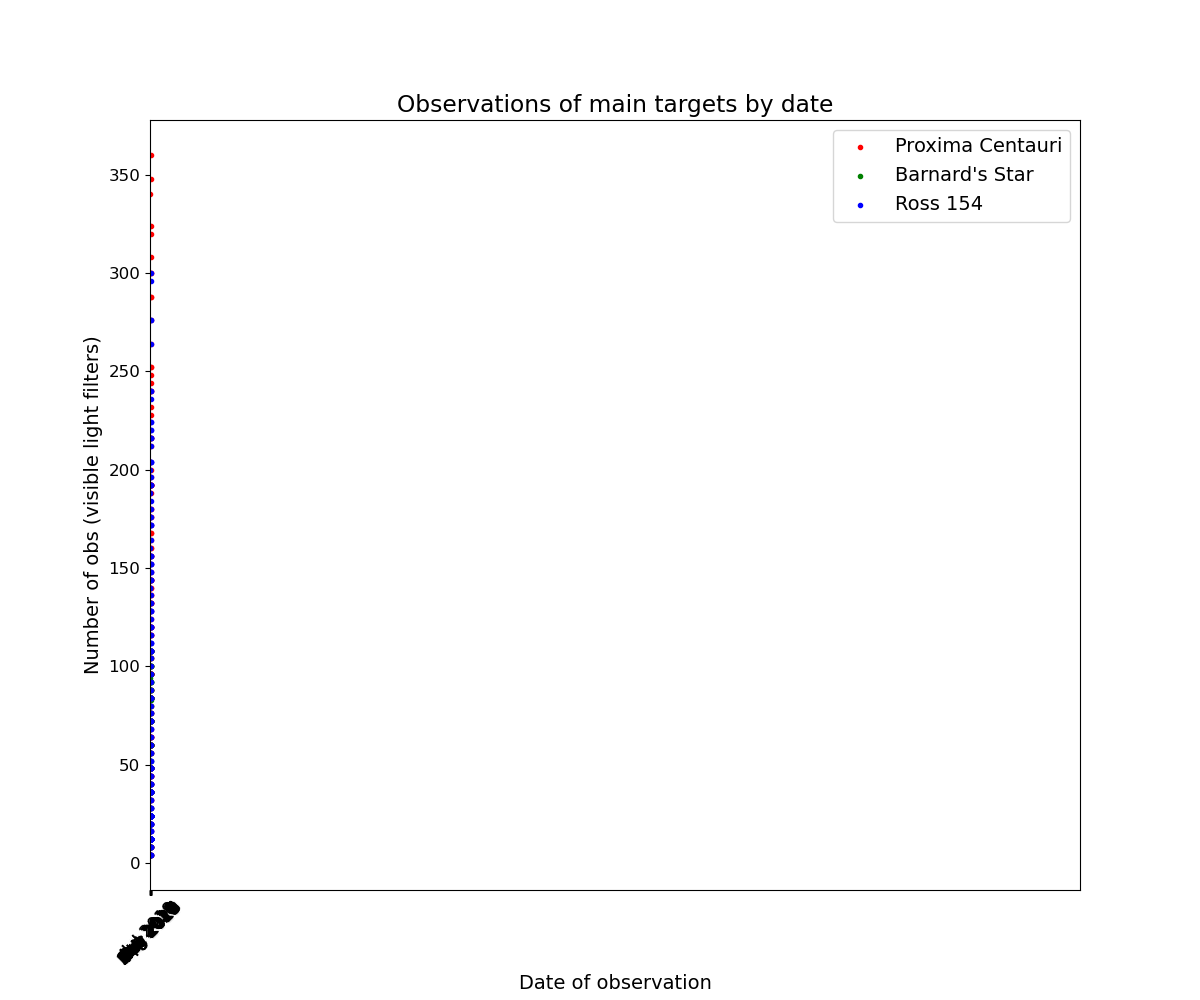
\includegraphics[scale=0.5]{images/visobstot.png} \\
\end{center}   
\caption{This figure shows the observations of the 3 target stars by date, as
of \date{\today}.}
\protect\label{fig:targobsplot}
\end{figure}
\subsection{Database and tools}
\protect\label{section:database}

To aid in the analysis of the data, a database was created using MySQL to
record and provide for fast retrieval of the objservational data, flat file
images and results, together with software tools and library routines in Python
and Perl.

The images were processed according to the formula:

\begin{center}
$ \frac{(mage - bias) \times mf}{flat - bias}$
\end{center}

In this $mf$ represents to mean value of the flat pixels. The mean value of the
master flat files is alleged to be 1 (in fact it is not after trimming off rows
and columns of the image containing zero or NaN values). The master flat files
already have the bias subtracted.

Half of the daily flat and bias files were made with a gain of 4.4, in line with
observations taken of targets other than the 3 main {\rdwarf} targets. As these
latter targets were all observed with a gain of 1, only the daily flat and bias
files with a gain of 1 were considered. The master bias files are
constructed from the daily bias files with a gain of 1.

\clearpage